\documentclass[]{article}

%Font encoding for swedish
\usepackage[utf8]{inputenc}
\usepackage[T1]{fontenc}

\usepackage{tabularx}

%Swedish
\usepackage[swedish]{babel}

%Concentrated lists
\usepackage{mdwlist}

\usepackage{multicol}

\usepackage{tocloft}

\usepackage{hyperref}

\usepackage{hyperref}
\hypersetup{hidelinks = true,}

\usepackage{tikz}
\usetikzlibrary{shapes,arrows,calc}

\usepackage[titletoc,title]{appendix}

\newcommand{\textoverline}[1]{$\overline{\mbox{#1}}$}

%opening
\title{Grafritande Räknare - Designskiss}
\author{Grupp 35:\\Hannes Haglund hanha265\\Felix Härnström felha423\\Silas Lenz sille914}

%Modifies toc spacing. Source: http://www.latex-community.org/forum/viewtopic.php?f=5&t=7701
\setlength\cftparskip{1pt}
\setlength\cftbeforesecskip{1pt}
\setlength\cftaftertoctitleskip{2pt}

\begin{document}

\pagenumbering{gobble}
\maketitle
%Making hspacing between toc entries smaller
%\renewcommand{\baselinestretch}{0.25}\normalsize
\tableofcontents
%\renewcommand{\baselinestretch}{1.0}\normalsize
\newpage
\pagenumbering{arabic}

\section{Översikt}
Vi ska implementera en generell dator av mikroprogrammerad, ej pipelinead typ. Mjukvaran skrivs i assembler. Vi har en VGA-motor, en tangentbordsavkodare och möjligtvis touchavkodare samt motor för dess skärm (utökningsmål). 

\tikzstyle{block} = [draw, fill=blue!20, rectangle, 
minimum height=3em, minimum width=6em]
\tikzstyle{sum} = [draw, fill=blue!20, circle, node distance=1cm]
\tikzstyle{input} = [coordinate]
\tikzstyle{output} = [coordinate]
\tikzstyle{pinstyle} = [pin edge={to-,thin,black}]

\begin{figure}[h]
\centering
\begin{tikzpicture}[auto, node distance=2cm,>=latex']



\node [block, node distance=3cm] (cpu) {CPU};
\node [block, below of=cpu, node distance=2cm] (memory) {Minne};
\node [output, right of=cpu] (foo) {};


\draw [<->] (cpu) -- node[near start]{} (memory);
\node [block, above of=cpu] (keyboarddriver) {Tangentbordsmotor};
\node [block, node distance=3.5cm, left of=keyboarddriver] (keyboard) {Tangentbord};

\draw [<->] (keyboarddriver) -- node {} (cpu);
\draw [->] (keyboard) -- node {} (keyboarddriver);

\node [block, node distance=2cm, below of=memory] (driver) {VGA-motor};
\node [block, right of=driver, node distance=3.5cm] (vga) {Skärm};
\draw [->] (memory) -- node {} (driver);
\draw [->] (driver) -- node {} (vga);
\draw[thick,dotted] ($(keyboarddriver.north west)+(-0.3,0.3)$)  rectangle ($(driver.south east)+(1,-0.3)$) node[pos=0] {FPGA};
\end{tikzpicture}
\caption{Översiktligt blockschema.}
\end{figure}

\newpage

\section{CPU}
Vår processor är mikroprogrammerad, med gemensamt data och programminne. Vi använder 32-bitars ordbredd. Endast blockram används.

Processor laddas alltid med samma program vid start. 

Nästan allt arbete utförs av processorn, förutom tangentbordläsning, och utritning av bildminnets innehåll. Dessa uppgifter inkluderar: beräkningar, historik, parsing av input, beräkning av graf, och så vidare.

Flyttalsupport ska finnas. Detta sköts i ALU:n snarare än i en separat flyttalsenhet; ett antal assembly-instruktioner, som använder sig av ALU:n, interpreterar indata (och utdata) som flyttal snarare än heltal. Konvertering från användarinmatade flyttal till flyttal i minnet sker via programkod.
\begin{figure}[h]
	\makebox[\textwidth][c]{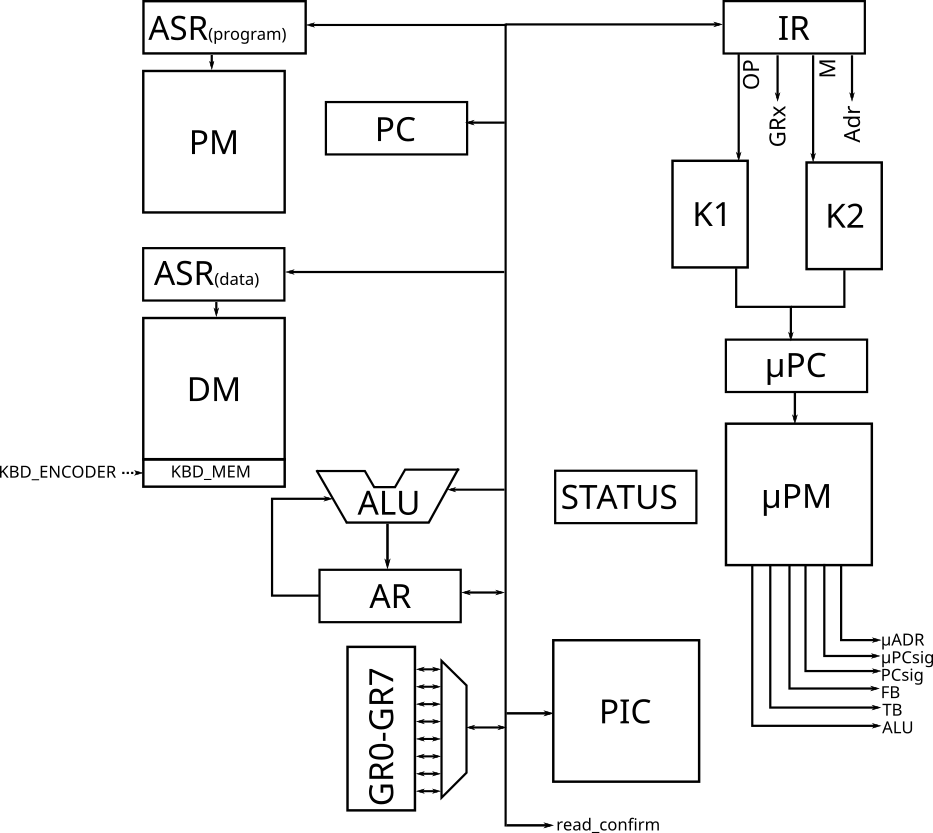
\includegraphics[width=1.2\textwidth]{cpu_v2.png}}
	\caption{Blockschema över CPU}
\end{figure}

\newpage

\section{Instruktioner}
Vi har följande adresseringsmoder:

%Hack to get a '2-column itemize'
\bigskip
\begin{tabular}{@{\textbullet\hspace*{\labelsep}}ll}
Direkt & (Binärkod \texttt{00}) \\
Omedelbar & (Binärkod \texttt{01}) \\
Indirekt & (Binärkod \texttt{10}) 
\end{tabular}
\bigskip

\noindent
Följande instruktionsmängd:

\begin{multicols}{5}
\begin{itemize*}
\item ADD
\item ADDF
\item SUB
\item SUBF
\item MULTF
\item DIVF
\item AND
\item ASL
\item ASR
\item BEQ
\item BMI
\item BNE
\item BRA
\item BRF
\item LOAD
\item STORE
\item HALT
\end{itemize*}
\end{multicols}

\noindent
En utförlig förklaring till varje instruktions argument, resultat, binärkod, adresseringsmoder, och påverkade flaggor finns tillgängligt som bilaga, på engelska.

I programminnet ges en instruktion på följande format:

\bigskip
\begin{tabular}{l|llll}
\textbf{Beskrivning} & Instruktion & Dataregister & Mod & Adress/literal \\
\textbf{Storlek} & 5 bitar & 3 bitar & 2 bitar & 22 bitar \\
%Exempel & \texttt{0001} & \texttt{101} & \texttt{01} &  \texttt{0000001011110110111100} \\
%Innebörd & SUB & Register 5 & Omedelbar & Värdet 48572 
\end{tabular}
\bigskip

\noindent
Om vi nu exempelvis skulle vilja subtrahera 48672 från värdet i register 5 skulle vi skriva följande i minnet:

\bigskip
\begin{tabular}{llll}
SUB & Register 5 & Omedelbar & Värdet 48572 \\
\texttt{01010} & \texttt{101} & \texttt{01} &  \texttt{0000001011110110111100}
\end{tabular}
\bigskip

\noindent
För mikrokodsinstruktionerna används följande format:

\bigskip
\begin{tabular}{l|llllll}
	\textbf{Beskrivning} & ALU     & Till buss & Från buss & PC    & SEQ & $\mu ADR $ \\
	\textbf{Storlek}     & 5 bitar & 4 bitar   & 4 bitar   & 1 bit & 4 bitar & 14 bitar
\end{tabular}
\bigskip
\newpage
\section{Grafik} 
Vi delar upp vår display i två kolumner, där ena hälften använder tiles och andra hälften använder en bitmap i svartvitt. Räknaren (text) använder sidan med tiles, och grafen använder bitmapsidan.

Upplösning 640x480. Både tiles och bitmap i svartvitt. Uppdateringsfrekvens 60Hz.

Processorn skriver tilenummer samt bitmapen direkt till bildminnet, utan att synkronisera med bilduppritningen.

\begin{figure}[h]
	\makebox[\textwidth][c]{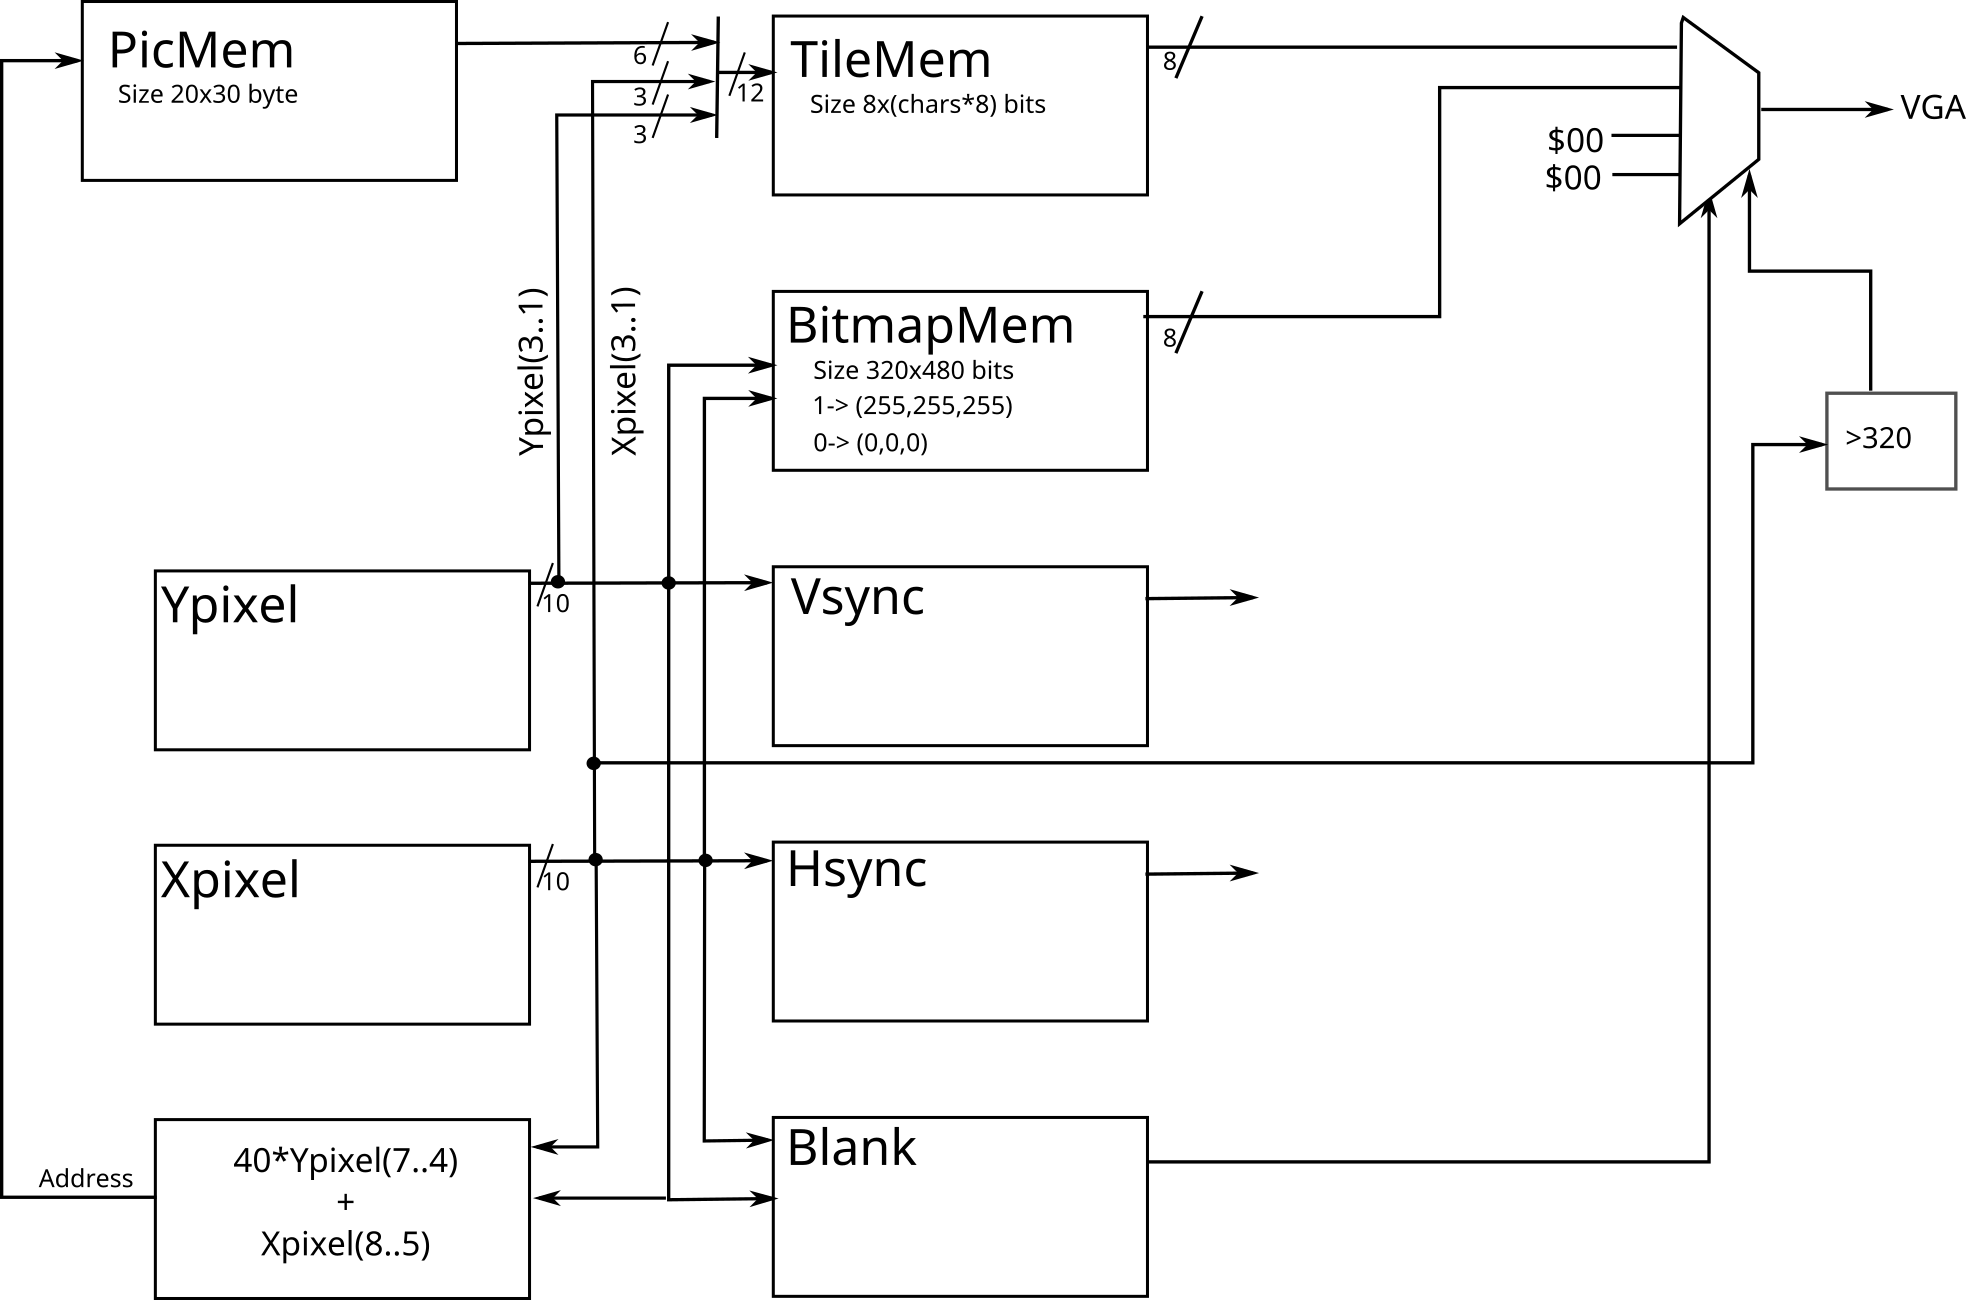
\includegraphics[width=1.2\textwidth]{vgamotor.png}}
	\caption{Blockschema över VGA-motor}
\end{figure}


\newpage

\section{I/O}
Input via PS/2 med en avkodare i \textsc{vhdl}. Avkodaren skriver ett tecken till en egen minnesplats som kan läsas av processorn via STORE. Vi låter instruktionen ta en virtuell adress som argument, och en viss adress som överskrider processorns minnesstorlek får referera till avkodarens minnescell.

Via en synkron \textit{read\_confirm}-signal så berättar processorn för avkodaren att den lyckats läsa ett tecken, varpå värdet på minnesplatsen nollställs.

Hämtad input ritas ut i ett konsolfönster på skärmen, och interpreteras vid nedslag av returknappen. Tal matas in i form av flyttal (separerad med punk), och uttryck skrivs i reverse-polish-notation.

\begin{figure}[h]
	\makebox[\textwidth][c]{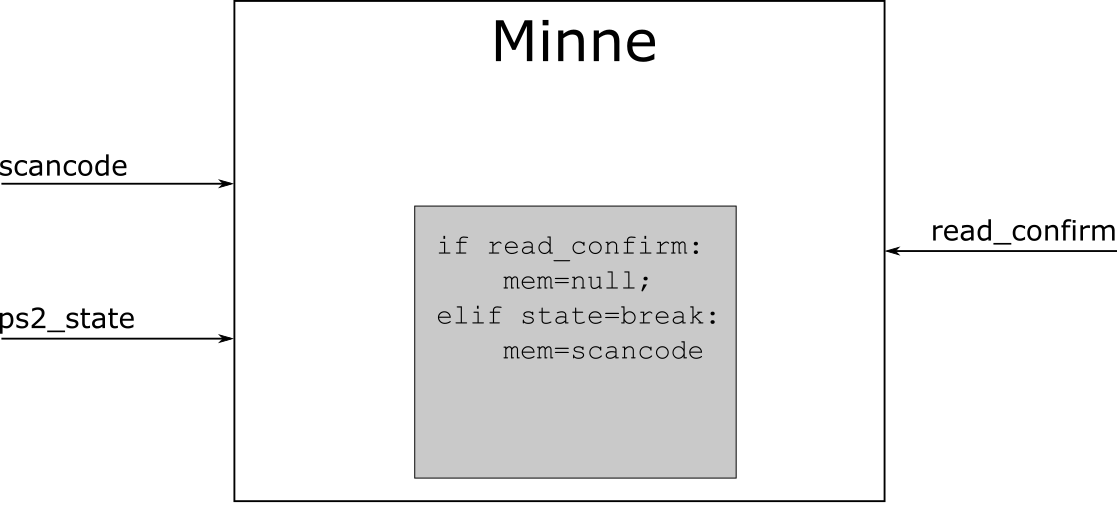
\includegraphics[width=1\textwidth]{io.png}}
	\caption{Blockschema över tangentbordsminne och read\_confirm - logik}
\end{figure}

\newpage

\section{Minne}
Vi har följande minnen:
\begin{itemize*}
\item PC (rw)
\item ASR (rw)
\item IR (rw)
\item $\mu$PC (rw)
\item $\mu$Minne (rw)
\item Programminne (rw)
\item 8 generella dataregister (rw)
\item Statusregister (r)
\item Bildminne
\item Bitmapminne
\item Tileminne
\item K1 (Instruktion -> $\mu$PC)
\item K2 (Mod -> $\mu$PC)
\end{itemize*}
Där program och dataminne använder ordlängden 32 bitar.

\section{Programmering}
Vi skriver en assembler, med lite syntaktiskt socker för loopar och if-satser.

\section{Milstolpe}
En fungerande processor som kan rita ut flyttal från en adress i minnet med hjälp av VGA-motor.

\clearpage
\begin{appendices}
\section{Instruktionsuppsättning}
Much of the instruction set is taken from the Motorola 68000 manual\footnote{\url{http://www.isy.liu.se/edu/kurs/TSEA82/kursmaterial/manual-68000.pdf}}.

%%%%%
% HALT
%%%%%
\noindent\rule{\textwidth}{1pt}\newline %Horizontal line
\newcolumntype{L}{>{\raggedright\arraybackslash}X} %Custom column type for left column
\setlength\extrarowheight{5pt} %Increase row spacing
\begin{tabularx}{\textwidth}{lL}
  {\Large \textbf{HALT}} 	& {\Large \textbf{Halt execution}}\\
  \textbf{Operation:} 		& \texttt{HALT}\\
  \textbf{Syntax:}  		& \texttt{HALT}\\
  \textbf{Binary code:} 	& \texttt{00000}\\
  \textbf{Description:}  	& Processor suspends all processing.\\
  \textbf{Condition codes:} & \texttt{X N Z V C\newline 0 0 0 0 0}\\
\end{tabularx}
\newline

%%%%%
% LOAD
%%%%%
\noindent\rule{\textwidth}{1pt}\newline %Horizontal line
\newcolumntype{L}{>{\raggedright\arraybackslash}X} %Custom column type for left column
\setlength\extrarowheight{5pt} %Increase row spacing
\begin{tabularx}{\textwidth}{lL}
  {\Large \textbf{LOAD}} 	& {\Large \textbf{Load value}}\\
  \textbf{Operation:} 		& \texttt{[data register] $\leftarrow$ <data>}\\
  \textbf{Syntax:}  		& \texttt{LOAD <ea>,Dn}\newline\texttt{LOAD \#<data>,Dn}\\
  \textbf{Binary code:} 	& \texttt{00001}\\
  \textbf{Description:}  	& Write to data register, where the data depends on the adressing mode. With direct adressing, it is the memory contents at the given address. With immediate, the given literal.\\
  \textbf{Condition codes:} & \texttt{X N Z V C\newline - - - - -}\\
\end{tabularx}
\newline

%%%%%
% STORE
%%%%%
\noindent\rule{\textwidth}{1pt}\newline %Horizontal line
\newcolumntype{L}{>{\raggedright\arraybackslash}X} %Custom column type for left column
\setlength\extrarowheight{5pt} %Increase row spacing
\begin{tabularx}{\textwidth}{lL}
  {\Large \textbf{STORE}} 	& {\Large \textbf{Store value}}\\
  \textbf{Operation:} 		& \texttt{[memory] $\leftarrow$ <data>}\\
  \textbf{Syntax:}  		& \texttt{STORE Dn,<ea>}\newline\texttt{STORE \#<data>,<ea>}\\
    \textbf{Binary code:} 	& \texttt{00010}\\
  \textbf{Description:}  	& Write to main memory. If a data register is given, its contents are written. If immediate addressing is used, a given literal is written.\\
  \textbf{Condition codes:} & \texttt{X N Z V C\newline - - - - -}\\
\end{tabularx}
\newline

\newpage

%%%%%
% BRA
%%%%%
\noindent\rule{\textwidth}{1pt}\newline %Horizontal line
\newcolumntype{L}{>{\raggedright\arraybackslash}X} %Custom column type for left column
\setlength\extrarowheight{5pt} %Increase row spacing
\begin{tabularx}{\textwidth}{lL}
  {\Large \textbf{BRA}} 	& {\Large \textbf{Branch always}}\\
  \textbf{Operation:} 		& \texttt{[PC] $\leftarrow$ [PC] + 1 + d}\\
  \textbf{Syntax:}  		& \texttt{BRA <label>}\newline\texttt{BRA <literal>}\\
  \textbf{Binary code:} 	& \texttt{00011}\\
  \textbf{Description:}  	& Program execution continues at location [PC] +1 + d.\\
  \textbf{Condition codes:} & \texttt{X N Z V C\newline - - - - -}\\
\end{tabularx}
\newline

%%%%%
% Bcc
%%%%%
\noindent\rule{\textwidth}{1pt}\newline %Horizontal line
\newcolumntype{L}{>{\raggedright\arraybackslash}X} %Custom column type for left column
\setlength\extrarowheight{5pt} %Increase row spacing
\begin{tabularx}{\textwidth}{lL}
  {\Large \textbf{Bcc}} 	& {\Large \textbf{Branch on condition cc}}\\
  \textbf{Operation:} 		& \texttt{If cc = 1 THEN [PC] $\leftarrow$ [PC] + 1 + d}\\
  \textbf{Syntax:}  		& \texttt{Bcc <label>}\\
  \textbf{Description:}  	& If the specified logical condition is met, program execution
continues at location [PC] + 1 + displacement, d.\newline

\texttt{BEQ} (\texttt{00100}) {} {} branch on equal\hfill \texttt{Z}\newline
\texttt{BMI} (\texttt{00101}) {} {} branch on minus\hfill \texttt{N}\newline
\texttt{BNE} (\texttt{00110}) {} {} branch on not equal\hfill \texttt{\textoverline{Z}}\newline
\texttt{BRF} (\texttt{00111}) {} {} branch on overflow set\hfill \texttt{V}\newline
\texttt{BPL} (\texttt{01000}) {} {} branch on plus\hfill \texttt{V}\newline
							  \\
  \textbf{Condition codes:} & \texttt{X N Z V C\newline - - - - -}\\
\end{tabularx}
\newline

\newpage

%%%%%
% ADD
%%%%%
\noindent\rule{\textwidth}{1pt}\newline %Horizontal line
\newcolumntype{L}{>{\raggedright\arraybackslash}X} %Custom column type for left column
\setlength\extrarowheight{5pt} %Increase row spacing
\begin{tabularx}{\textwidth}{lL}
  {\Large \textbf{ADD}} 	& {\Large \textbf{Signed integer add}}\\
  \textbf{Operation:} 		& \texttt{[destination] $\leftarrow$ [source] + [destination]}\\
  \textbf{Syntax:}  		& \texttt{ADD <ea>,Dn}\newline\texttt{ADD Dn,<ea>}\newline\texttt{ADD \#<value>,Dn}\\
  \textbf{Binary code:} 	& \texttt{01001}\\
  \textbf{Description:}  	& Add the source operand to the destination operand and store the
result in the destination location. The source can be given as a literal using immediate addressing.\\
  \textbf{Condition codes:} & \texttt{X N Z V C\newline * * * * *}\newline\newline The X-bit and C-bit are both set if carry is generated. The N-bit is set if the sum is negative. The Z-bit is set if the sum is zero. The V-bit is set if overflow occurs (in which case the Z-bit and the N-bit are undefined).\\
\end{tabularx}
\newline

%%%%%
% ADDF
%%%%%
\noindent\rule{\textwidth}{1pt}\newline %Horizontal line
\newcolumntype{L}{>{\raggedright\arraybackslash}X} %Custom column type for left column
\setlength\extrarowheight{5pt} %Increase row spacing
\begin{tabularx}{\textwidth}{lL}
  {\Large \textbf{ADDF}} 	& {\Large \textbf{Signed floating-point add}}\\
  \textbf{Operation:} 		& \texttt{[destination] $\leftarrow$ [source] + [destination]}\\
  \textbf{Syntax:}  		& \texttt{ADDF <ea>,Dn}\newline\texttt{ADDF Dn,<ea>}\newline\texttt{ADDF \#<value>,Dn}\\
  \textbf{Binary code:} 	& \texttt{01010}\\
  \textbf{Description:}  	& Add the source operand to the destination operand and store the
result in the destination location, interpreting operands and sum as signed floating-point numbers. The source can be given as a literal using immediate addressing.\\
  \textbf{Condition codes:} & \texttt{X N Z V C\newline * * * * *}\newline\newline The X-bit and C-bit are both set if carry is generated. The N-bit is set if the sum is negative. The Z-bit is set if the sum is zero. The V-bit is set if overflow occurs (in which case the Z-bit and the N-bit are undefined).\\
\end{tabularx}
\newline

\newpage

%%%%%
% SUB
%%%%%
\noindent\rule{\textwidth}{1pt}\newline %Horizontal line
\newcolumntype{L}{>{\raggedright\arraybackslash}X} %Custom column type for left column
\setlength\extrarowheight{5pt} %Increase row spacing
\begin{tabularx}{\textwidth}{lL}
  {\Large \textbf{SUB}} 	& {\Large \textbf{Signed integer subtract}}\\
  \textbf{Operation:} 		& \texttt{[destination] $\leftarrow$ [source] - [destination]}\\
  \textbf{Syntax:}  		& \texttt{SUB <ea>,Dn}\newline\texttt{SUB Dn,<ea>}\newline\texttt{SUB \#<value>,Dn}\\
  \textbf{Binary code:} 	& \texttt{01011}\\
  \textbf{Description:}  	& Subtract the destination operand from the source operand and store the
result in the destination location. The source can be given as a literal using immediate addressing.\\
  \textbf{Condition codes:} & \texttt{X N Z V C\newline * * * * *}\newline\newline The X-bit and C-bit are both set if carry is generated. The N-bit is set if the difference is negative. The Z-bit is set if the difference is zero. The V-bit is set if overflow occurs (in which case the Z-bit and the N-bit are undefined).\\
\end{tabularx}
\newline

%%%%%
% SUBF
%%%%%
\noindent\rule{\textwidth}{1pt}\newline %Horizontal line
\newcolumntype{L}{>{\raggedright\arraybackslash}X} %Custom column type for left column
\setlength\extrarowheight{5pt} %Increase row spacing
\begin{tabularx}{\textwidth}{lL}
  {\Large \textbf{SUBF}} 	& {\Large \textbf{Signed floating-point subtract}}\\
  \textbf{Operation:} 		& \texttt{[destination] $\leftarrow$ [source] - [destination]}\\
  \textbf{Syntax:}  		& \texttt{SUBF <ea>,Dn}\newline\texttt{SUBF Dn,<ea>}\newline\texttt{SUBF \#<value>,Dn}\\
  \textbf{Binary code:} 	& \texttt{01100}\\
  \textbf{Description:}  	& Subtract the destination operand from the source operand and store the
result in the destination location, interpreting operands and difference as signed floating-point numbers. The source can be given as a literal using immediate addressing.\\
  \textbf{Condition codes:} & \texttt{X N Z V C\newline * * * * *}\newline\newline The X-bit and C-bit are both set if carry is generated. The N-bit is set if the difference is negative. The Z-bit is set if the difference is zero. The V-bit is set if overflow occurs (in which case the Z-bit and the N-bit are undefined).\\
\end{tabularx}
\newline

\newpage

%%%%%
% DIVF
%%%%%
\noindent\rule{\textwidth}{1pt}\newline %Horizontal line
\newcolumntype{L}{>{\raggedright\arraybackslash}X} %Custom column type for left column
\setlength\extrarowheight{5pt} %Increase row spacing
\begin{tabularx}{\textwidth}{lL}
  {\Large \textbf{DIVF}} 	& {\Large \textbf{Signed floating-point divide}}\\
  \textbf{Operation:} 		& \texttt{[destination] $\leftarrow$ [destination] / [source]}\\
  \textbf{Syntax:}  		& \texttt{DIVF <ea>,Dn}\newline\texttt{DIVF \#<value>,Dn}\\
  \textbf{Binary code:} 	& \texttt{01101}\\
  \textbf{Description:}  	& Divide the destination operand by the source operand and store
the result in the destination, interpreting operands and result as signed floating-point numbers.\\
  \textbf{Condition codes:} & \texttt{X N Z V C\newline - * * * 0}\newline\newline The X-bit is not affected by a division. The N-bit is set if the
quotient is negative. The Z-bit is set if the quotient is zero. The Vbit
is set if division overflow occurs (in which case the Z- and Nbits
are undefined). The C-bit is always cleared.\\
\end{tabularx}
\newline

%%%%%
% MULTF
%%%%%
\noindent\rule{\textwidth}{1pt}\newline %Horizontal line
\newcolumntype{L}{>{\raggedright\arraybackslash}X} %Custom column type for left column
\setlength\extrarowheight{5pt} %Increase row spacing
\begin{tabularx}{\textwidth}{lL}
  {\Large \textbf{MULTF}} 	& {\Large \textbf{Signed floating-point multiply}}\\
  \textbf{Operation:} 		& \texttt{[destination] $\leftarrow$ [destination] $\times$ [source]}\\
  \textbf{Syntax:}  		& \texttt{MULTF <ea>,Dn}\newline\texttt{MULTF \#<value>,Dn}\\
  \textbf{Binary code:} 	& \texttt{01110}\\
  \textbf{Description:}  	& Multiply the destination operand by the source operand and store
the result in the destination, interpreting operands and result as signed floating-point numbers. The source can be given as a literal using immediate addressing.\\
  \textbf{Condition codes:} & \texttt{X N Z V C\newline - * * * 0}\newline\newline The X-bit is not affected by a multiplication. The N-bit is set if the 
product is negative. The Z-bit is set if the product is zero. The V-bit
is set if division overflow occurs (in which case the Z-bit and the N-bit
are undefined). The C-bit is always cleared.\\
\end{tabularx}
\newline

\newpage

%%%%%
% AND
%%%%%
\noindent\rule{\textwidth}{1pt}\newline %Horizontal line
\newcolumntype{L}{>{\raggedright\arraybackslash}X} %Custom column type for left column
\setlength\extrarowheight{5pt} %Increase row spacing
\begin{tabularx}{\textwidth}{lL}
  {\Large \textbf{AND}} 	& {\Large \textbf{Logical AND}}\\
  \textbf{Operation:} 		& \texttt{[destination] $\leftarrow$ [source].[destination]}\\
  \textbf{Syntax:}  		& \texttt{AND <ea>,Dn}\newline\texttt{AND Dn,<ea>}\newline\texttt{AND \#<value>,Dn}\\
  \textbf{Binary code:} 	& \texttt{01111}\\
  \textbf{Description:}  	& AND the source operand to the destination operand and store the
result in the destination location. The source can be given as a literal using immediate addressing.\\
  \textbf{Condition codes:} & \texttt{X N Z V C\newline - * * 0 0}\newline\newline The N-bit is set to the most significant bit of the result. The Z-bit is set if the result is equal to zero.\\
\end{tabularx}
\newline

\newpage

%%%%%
% ASL/ASR
%%%%%
\noindent\rule{\textwidth}{1pt}\newline %Horizontal line
\newcolumntype{L}{>{\raggedright\arraybackslash}X} %Custom column type for left column
\setlength\extrarowheight{5pt} %Increase row spacing
\begin{tabularx}{\textwidth}{lL}
  {\Large \textbf{ASL/ASR}} 	& {\Large \textbf{Arithmetic shift left/right}}\\
  \textbf{Operation:} 		& \texttt{[destination] $\leftarrow$ [destination] shifted by <count>}\\
  \textbf{Syntax:}  		& \texttt{ASL <ea>,Dn}\newline
  							  \texttt{ASR <ea>,Dn}\newline
 							  \texttt{ASL \#<data>,Dy}\newline
 							  \texttt{ASR \#<data>,Dy}\newline							  
 							  \\
  \textbf{Binary code:} 	& ASL: \texttt{10000}, ASR: \texttt{10001}\\
  \textbf{Description:}  	& Arithmetically shift the bits of the operand in the specified direction
(i.e., left or right). The shift count may be specified in one of
three ways. The count may be a literal, the contents of a data
register, or the value 1. An immediate (i.e., literal) count permits
a shift of 1 to 8 places. If the count is in a register, the value is
modulo 64 (i.e., 0 to 63). If no count is specified, one shift is made
(i.e., ASL <ea> shifts the contents of the word at the effective
address one place left).

The effect of an arithmetic shift left is to shift a zero into the
least-significant bit position and to shift the most-significant bit
out into both the X- and the C-bits of the CCR. The overflow bit
of the CCR is set if a sign change occurs during shifting (i.e., if
the most-significant bit changes value during shifting).

The effect of an arithmetic shift right is to shift the least significant
bit into both the X- and C-bits of the CCR. The mostsignificant
bit (i.e., the sign bit) is replicated to preserve the sign of
the number.\\
  \textbf{Condition codes:} & \texttt{X N Z V C\newline * * * * *}\newline The X-bit and the C-bit are set according to the last bit shifted out
of the operand. If the shift count is zero, the C-bit is cleared.\\
\end{tabularx}
\newline

\newpage

%%%%%
% JMP
%%%%%
\noindent\rule{\textwidth}{1pt}\newline %Horizontal line
\newcolumntype{L}{>{\raggedright\arraybackslash}X} %Custom column type for left column
\setlength\extrarowheight{5pt} %Increase row spacing
\begin{tabularx}{\textwidth}{lL}
  {\Large \textbf{JMP}} 	& {\Large \textbf{Jump}}\\
  \textbf{Operation:} 		& \texttt{[PC] $\leftarrow$ d}\\
  \textbf{Syntax:}  		& \texttt{JMP <label>}\newline\texttt{JMP <literal>}\\
  \textbf{Binary code:} 	& \texttt{10111}\\
  \textbf{Description:}  	& Program execution continues at location d.\\
  \textbf{Condition codes:} & \texttt{X N Z V C\newline - - - - -}\\
\end{tabularx}
\newline

%%%%%
% LSL/LSR
%%%%%
\noindent\rule{\textwidth}{1pt}\newline %Horizontal line
\newcolumntype{L}{>{\raggedright\arraybackslash}X} %Custom column type for left column
\setlength\extrarowheight{5pt} %Increase row spacing
\begin{tabularx}{\textwidth}{lL}
  {\Large \textbf{LSL/LSR}} 	& {\Large \textbf{Logical shift left/right}}\\
  \textbf{Operation:} 		& \texttt{[destination] $\leftarrow$ [destination] shifted by <count>}\\
  \textbf{Syntax:}  		& \texttt{LSL <ea>,Dn}\newline
  							  \texttt{LSR <ea>,Dn}\newline
 							  \texttt{LSL \#<data>,Dy}\newline
 							  \texttt{LSR \#<data>,Dy}\newline						  
 							  \\
  \textbf{Binary code:} 	& LSR: \texttt{10101}, LSL: \texttt{10110}\\
  \textbf{Description:}  	& Logically shift the bits of the operand in the specified direction
(i.e., left or right). A zero is shifted into the input position and the
bit shifted out is copied into both the C- and the X-bit of the CCR.
The shift count may be specified in one of three ways. The count
may be a literal, the contents of a data register, or the value 1. An
immediate count permits a shift of 1 to 8 places. If the count is in
a register, the value is modulo 64  from 0 to 63. If no count is
specified, one shift is made (e.g., LSL <ea> shifts the word at the
effective address one position left).\\
  \textbf{Condition codes:} & \texttt{X N Z V C\newline * * * 0 *}\newline The X-bit is set to the last bit shifted out of the operand and is
equal to the C-bit. However, a zero shift count leaves the X-bit
unaffected and the C-bit cleared.\\
\end{tabularx}
\newline

\newpage

%%%%%
% STOREP
%%%%%
\noindent\rule{\textwidth}{1pt}\newline %Horizontal line
\newcolumntype{L}{>{\raggedright\arraybackslash}X} %Custom column type for left column
\setlength\extrarowheight{5pt} %Increase row spacing
\begin{tabularx}{\textwidth}{lL}
  {\Large \textbf{STOREP}} 	& {\Large \textbf{Store to pictmem}}\\
  \textbf{Operation:} 		& \texttt{Pictmem[d] $\leftarrow$ GRx}\\
  \textbf{Syntax:}  		& \texttt{STOREP <ea>,Dn}\\
  \textbf{Binary code:} 	& \texttt{10111}\\
  \textbf{Description:}  	& Stores the character (as tile index) in given register to pictmem at given address.\\
  \textbf{Condition codes:} & \texttt{X N Z V C\newline - - - - -}\\
\end{tabularx}
\newline

%%%%%
% RC
%%%%%
\noindent\rule{\textwidth}{1pt}\newline %Horizontal line
\newcolumntype{L}{>{\raggedright\arraybackslash}X} %Custom column type for left column
\setlength\extrarowheight{5pt} %Increase row spacing
\begin{tabularx}{\textwidth}{lL}
  {\Large \textbf{RC}} 	& {\Large \textbf{Read character}}\\
  \textbf{Operation:} 		& \texttt{GRx $\leftarrow$ character from keyboard}\\
  \textbf{Syntax:}  		& \texttt{RC Dn}\\
  \textbf{Binary code:} 	& \texttt{11000}\\
  \textbf{Description:}  	& Stores the currently pressed character from keyboard to given register.\\
  \textbf{Condition codes:} & \texttt{X N Z V C\newline - - - - -}\\
\end{tabularx}
\newline

%%%%%
% CMP
%%%%%
\noindent\rule{\textwidth}{1pt}\newline %Horizontal line
\newcolumntype{L}{>{\raggedright\arraybackslash}X} %Custom column type for left column
\setlength\extrarowheight{5pt} %Increase row spacing
\begin{tabularx}{\textwidth}{lL}
  {\Large \textbf{CMP}} 	& {\Large \textbf{Compare}}\\
  \textbf{Operation:} 		& \texttt{[destination] - [source]}\\
  \textbf{Syntax:}  		& \texttt{CMP <ea>,Dn}\\
  \textbf{Binary code:} 	& \texttt{11000}\\
  \textbf{Description:}  	& Subtract the source operand from the destination operand and set the condition codes accordingly. The destination must be a data register. The destination is not modified by this instruction.\\
  \textbf{Condition codes:} & \texttt{X N Z V C\newline - * * * *}\\
\end{tabularx}
\newline

\end{appendices}
\end{document}
